\question \textbf{Tossing Coins} \\*
A fair coin is tossed repeatedly and independently. Find the expected 
number of tosses till the pattern HTH appears.
\begin{solution}[6cm]
Call HTH our target. Consider a chain that starts from a state called 
nothing $(\emptyset)$ and is eventually absorbed at HTH. If we first 
toss H then we move to state H because this is the first letter of our 
target. If we toss a T then we move back to $\emptyset$ having expended 
1 unit of time. Being in state H we either move to a new state HT if 
we bring T and we are 1 step closer to the target or, if we bring H, 
we move back to H: we have expended 1 unit of time, but the new H can 
be the beginning of a target. When in state HT we either move to HTH 
and we are done or, if T occurs then we move to $\emptyset$. The 
transition diagram is

\begin{center}
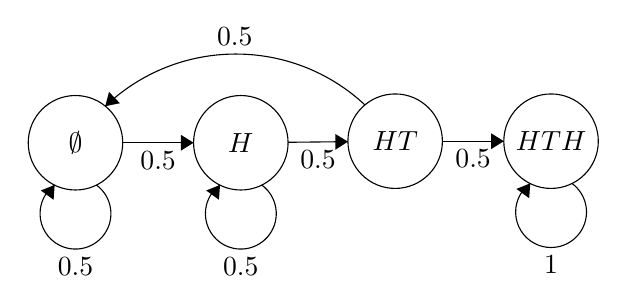
\begin{tikzpicture}[scale=0.2]
\tikzstyle{every node}+=[inner sep=0pt]
\draw [black] (16.9,-32.7) circle (3);
\draw (16.9,-32.7) node {$\emptyset$};
\draw [black] (27.4,-32.7) circle (3);
\draw (27.4,-32.7) node {$H$};
\draw [black] (37.2,-32.6) circle (3);
\draw (37.2,-32.6) node {$HT$};
\draw [black] (47.1,-32.6) circle (3);
\draw (47.1,-32.6) node {$HTH$};
\draw [black] (18.223,-35.38) arc (54:-234:2.25);
\draw (16.9,-39.95) node [below] {$0.5$};
\fill [black] (15.58,-35.38) -- (14.7,-35.73) -- (15.51,-36.32);
\draw [black] (19.9,-32.7) -- (24.4,-32.7);
\fill [black] (24.4,-32.7) -- (23.6,-32.2) -- (23.6,-33.2);
\draw (22.15,-33.2) node [below] {$0.5$};
\draw [black] (28.723,-35.38) arc (54:-234:2.25);
\draw (27.4,-39.95) node [below] {$0.5$};
\fill [black] (26.08,-35.38) -- (25.2,-35.73) -- (26.01,-36.32);
\draw [black] (30.4,-32.67) -- (34.2,-32.63);
\fill [black] (34.2,-32.63) -- (33.4,-32.14) -- (33.41,-33.14);
\draw (32.3,-33.17) node [below] {$0.5$};
\draw [black] (18.793,-30.382) arc (133.61233:46.95216:12.017);
\fill [black] (18.79,-30.38) -- (19.72,-30.19) -- (19.03,-29.47);
\draw (27.02,-26.56) node [above] {$0.5$};
\draw [black] (40.2,-32.6) -- (44.1,-32.6);
\fill [black] (44.1,-32.6) -- (43.3,-32.1) -- (43.3,-33.1);
\draw (42.15,-33.1) node [below] {$0.5$};
\draw [black] (48.423,-35.28) arc (54:-234:2.25);
\draw (47.1,-39.85) node [below] {$1$};
\fill [black] (45.78,-35.28) -- (44.9,-35.63) -- (45.71,-36.22);
\end{tikzpicture}

Let $\phi(i)$ be the expected number of steps to reach HTH starting 
from $i$. We have 

\begin{align*}
\phi(HT) &= 1 + \frac{1}{2} \phi(\emptyset) \\
\phi(H) &= 1 + \frac{1}{2} \phi(H) + \frac{1}{2} \phi(HT) \\
\phi(\emptyset) &= 1 + \frac{1}{2} \phi(\emptyset) + \frac{1}{2} \phi(H)
\end{align*}
We solve and find $\phi(\emptyset) = 10$.
\end{center}

\end{solution}